\chapter{Prototyp}\label{ch:prototype}
\section{Cele i zakres}
Jako początkowy etap przygotowania projektu stworzono prototyp gry. Został on przygotowany w kilku celach.
\begin{enumerate}
    \item Zapoznanie z możliwościami i ograniczeniami silnika. 
    \item Określenie trudności przygotowania warstwy sieciowej.
    \item Zapoznanie z językiem skryptowym GDScript. 
\end{enumerate}

W ramach prototypu zaimplementowano jedynie bardzo podstawowe mechaniki: poruszanie, celowanie i strzelanie. System sieciowy również zaimplementowano w uproszczonej formie, nie implementując również wszystkich mechanik sieciowo - jedynie poruszanie i celowanie.

Na tym etapie nie przygotowano żadnych grafik, jako modele i poziom zostały wykorzystane jedynie proste figury geometryczne generowane w silniku.

\section{Mechaniki}
W ramach prototypu wprowadzone zostały implementacje poruszania/sterowania, celowania i strzelania.

\subsection{Przygotowanie projektu}
Tworzenie projektu rozpoczęto od przygotowania świata gry oraz postaci gracza, w celu umożliwienia testowania oprogramowania. 

Świat gry został zbudowany z przeskalowanych prostopadłościanów działających jako podłoże, ściany ograniczające poziom oraz przeszkody w poziomie. Wykorzystano również figury CSG (\emph{Constructive Solid Geometry} - ang. Konstrulcyjna Geometria Bryłowa) w celu stworzenia bardziej skomplikowanej przeszkody. Bryły tego rodzaju można łączyć w spójne figury z pomocą takich operacji jak suma, różnica czy część wspólna.

Awatar gracza został złożony z dwóch części - ciała (ang. \emph{body}) i głowy (ang. \emph{head}). Są to jedynie nazwy dla prostego rozróżnienia kadłuba od wieżyczki wraz z lufą. Taki podział został wprowadzony w celu prostszego i niezależego sterowania transformacją oraz rotacją tych elementów. Całość została przygotowana z wykorzystaniem trzech brył - prostopadłościanu dla ciała, kuli dla wieżyczki oraz walca dla lufy.


\subsection{Poruszanie}
Został wprowadzony schemat sterowania zgodny z ustaleniami sekcji \ref{sec:steering_concept} oraz tabeli \ref{tab:steering}. 

Postać gracza poruszana jest jedynie w przypadku jeżeli odpowiedni przycisk jest przytrzymywany. W tym celu w procesie fizycznym wykonywane jest sprawdzenie wprowadzanych przez gracza poleceń. 

Proces fizyczny to metoda w skryptach Godota, wywoływana co ustalony czas, niezależny od wyświetlanych klatek. Pozwala to na ujednolicenie działania krytycznych części kodu w przypadku gdy scena i klatka może być generowana dłużej niż zwykle.

Ponieważ ruch w osi przód-tył i obrót w prawo-lewo są różnymi zachowaniami wejścia z nimi związane zostały zapisane do oddzielnych zmiennych. Ponadto, ponieważ jednoczesny obrót lub ruch w obie strony się wykluczają, wartość tych dwóch poleceń zostaje od siebie odjęta. \ref{lst:getting_input}

\begin{lstlisting}[language=python,caption=Kod pobierający polecenia gracza, label=lst:getting_input,basicstyle=\footnotesize\ttfamily]
var forward_input = int(Input.is_action_pressed("Forward")) 
  - int(Input.is_action_pressed("Back"))
var turn_input = int(Input.is_action_pressed("Left")) 
  - int(Input.is_action_pressed("Right"))
\end{lstlisting}

\texttt{Input} jest obiektem tworzonym przez silnik, singletonem, który zarządza interfejsami poleceń gracza takimi jak klawiatura i mysz. Zamiast metody \texttt{is\_action\_pressed}, która sprawdza aktualny stan akcji, możliwe jest również wykorzystanie metody \texttt{get\_axis}, która pozwala skrócić powyższy zapis zachowując ten sam rezultat. Odpowiednie akcje zostały stworzone i zmapowane do odpowiednich wejść z tabeli \ref{tab:steering}, korzystając z mapowania wejścia w ustawieniach projektu Godota.

W skrypcie gracza zdefiniowane zostały atrybuty niezbędne do implementacji poruszania - prędkość maksymalna i aktualna poruszania oraz prędkość kątowa maksymalna i aktualna obrotu. Aktualna prędkość poruszania jest wartością wektorową, pozostałe zaś są wartościami skalarnymi. Zmienne przechowujące wartości maksymalne są zdefiniowane wykorzystaniem słowa kluczowego \texttt{export} co pozwala na edytowanie ich w oknie silnika Godot.

Jako oś przód-tył wykorzystano oś $z$ modelu gracza, gdzie przód jest zwrócony zgodnie z dodatnią częścią osi. W celu poruszenia całego obiektu gracza wywołana zostaje funkcja \texttt{move\_and\_slide}, która służy do przemieszczania obiektów z uwzględnieniem kolizji. Do obrócenia modelu wykorzystano metodę \texttt{rotate\_y}, ponieważ w silniku Godot oś ``y'' jest osią pionową.

Została podjęta decyzja o wykorzystaniu kamery trzecioosobowej, tj. takiej, która podąża za graczem i widzi również jego model, w odróżnieniu od kamery pierwszoosobowej, która widzi świat z perspektywy gracza. Wybrano wbudowaną w silnik Godot kamerę interpolowaną (\texttt{InterpolatedCamera}). Jest to kamera, która porusza się płynnie tak, aby jej położenie pokrywało się z jej celem. Cel kamery jest również obiektem o odpowiedniej pozycji i rotacji.

Cel oraz kamera zostały dodane do sceny świata, a nie gracza, aby na etapie dodawania systemu sieciowego (\ref{sec:network_prototype}) móc uniknąć problemu wielu niewykorzystanych obiektów. 

W skrypcie świata, w procesie fizycznym cel kamery jest przenoszony w pozycję o odpowiednich koordynatach. kamera będzie automatycznie przemieszczała się tak, aby śledzić ten punkt, jednak jej rotacja również ustawiana programistycznie, poprzez wykorzystanie metody \texttt{look\_at}. 

\subsection{Celowanie}

Celowanie zostało zaimplementowane zgodnie z sekcją \ref{sec:shooting_concept}. W tym celu należy wykonać następujące kroki:
\begin{enumerate}
    \item\label{pt:get_mouse} Pobrać pozycję myszy w oknie gry;
    \item Pobrać pozycję kamery w świecie gry;
    \item Wyznaczyć promień przechodzący od kamery w kierunku wskazywanym przez mysz;
    \item\label{pt:get_ray_intersection} Zbadać przecięcia powyższego promienia z obiektami świata gry;
    \item Wycelować w kierunku wyznaczonego punktu przecięcia.  
\end{enumerate}

Kod funkcji realizującej punkty \ref{pt:get_mouse}-\ref{pt:get_ray_intersection} został zamieszczony w listingu \ref{lst:mouse_to_world}.

\begin{lstlisting}[language=python,caption=Funkcja rzutująca mysz na świat gry, label=lst:mouse_to_world,basicstyle=\footnotesize\ttfamily]
func mousePositionToWorldPosition():
  var space_state = get_world().direct_space_state
  var mouse_pos = get_viewport().get_mouse_position()

  var camera = get_tree().root.get_camera()
  if camera == null:
    return null

  var ray_origin = camera.global_translation
  var ray_direction = camera.project_position(mouse_pos, 300)

  var ray_array = space_state.intersect_ray(ray_origin, ray_direction)

  if ray_array.has("position"):
    return ray_array["position"]
  return null
\end{lstlisting}

Jeżeli zostanie znaleziony punkt przecięcia promienia z obiektami świata, cała ``głowa'' modelu gracza jest obracana w jego kierunku. W prototypie punkt ten jest również wizualizowany kulą, która się w nim pojawia. Pomogło to w zniwelowaniu błędów wynikających z różnicy między przestrzenią lokalną modelu gracza a globalną. 

\subsection{Strzelanie}
Stworzony został obiekt pocisku. Jego modelem jak i kształtem kolizji jest figura kapsuły. 

Jako część postaci gracza dodany został węzeł typu \texttt{Spatial} reprezentujący punkt, w którym tworzone będą pociski. Został on umieszczony na końcu lufy i przypisany jako dziecko tego obiektu. W ten sposób punkt ten będzie przemieszczał się tak samo jak jego rodzic. Do skryptu gracza została również dodana zmienna przechowująca referencję do sceny pocisku.

Do skryptu gracza dodano także funkcję strzału, oraz kod przyjmujący polecenie strzału z myszy. Podobnie jak akcje poruszania, akcja strzału została zmapowana w ustawieniach projektu. Z perspektywy gracza strzał polega jedynie na stworzeniu instancji sceny pocisku, umieszczeniu jej w punkcie strzału na końcu lufy oraz przypisaniu jej do świata gry. Pociski nie mogą być zapisywane jako dzieci gracza, ponieważ wtedy przemieszczałyby się razem z nim.

Do skryptu pocisku dodano stałe określające szybkość poruszania oraz limit czasu istnienia obiektu. W momencie utworzenia instancji pocisku licznik czasu istnienia zaczyna odliczać liczbę sekund równą limitowi. W przypadku zakończenia licznika obiekt pocisku jest niszczony. W procesie fizycznym pocisk przemieszczany jest z odpowiednią szybkością w jego lokalnym kierunku $+z$. Po wykryciu zderzenia pocisk jest niszczony.   

\section{System sieciowy}\label{sec:network_prototype}

Podstawowy system sieciowy został zaimplementowany z wykorzystaniem wideoporadnika \cite{godot_network_tutorial}. Ostateczna implementacja została jednak dostosowana do przygotowywanego rozwiązania, ponieważ projekt z poradnika jest tworzony z wykorzystaniem grafiki 2D.

Do projektu dodano pusty węzeł statyczny mający przechowywać graczy w drzewie. Ponadto dodano menu startowe (Rys. \ref{fig:prototype_menu}). Stworzono również dwa skrypty globalne oraz zmodyfikowano skrypt gracza.

\begin{figure}
    \centering
    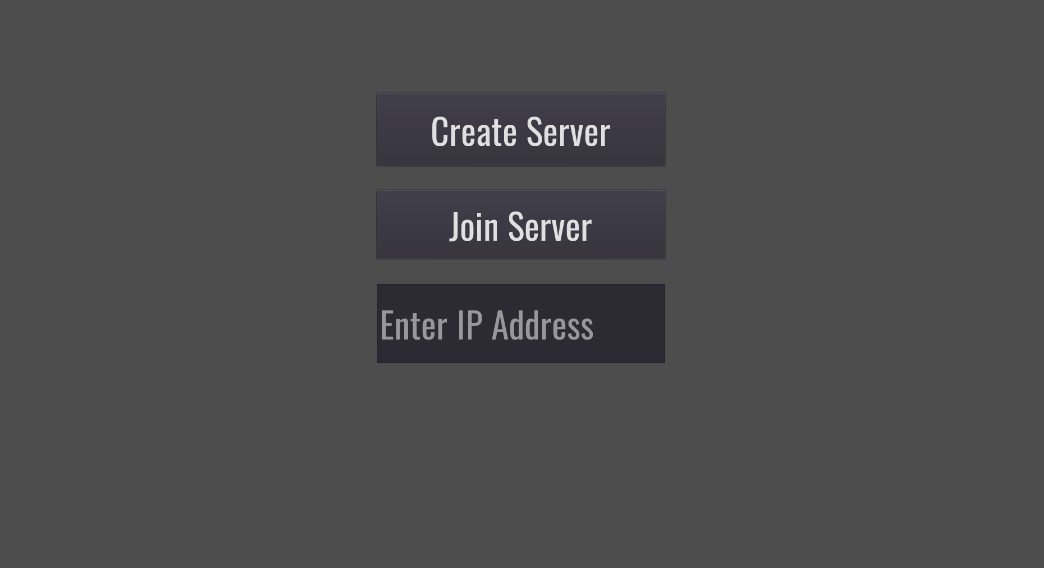
\includegraphics[width=.9\linewidth]{Images/prototype/prototype_net_menu.png}
    \caption{Menu startowe prototypu po wprowadzeniu systemu sieciowego}
    \label{fig:prototype_menu}
\end{figure}

Na interfejsie menu widoczne są dwa przyciski. Przycisk ``Create Server'' powoduje rozpoczęcie gry jako host. Gra hostowana jest wtedy na adresie IP maszyny użytkownika. Przycisk ``Join Server'' powoduje rozpoczęcie gry na serwerze, którego adres IP wpisany jest w pole tekstowe. W prototypie nie zostały zastosowane żadne techniki obrony przed wpisaniem niepoprawnego adresu IP ani próby połączenia z nieistniejącym serwerem.

Skrypt globalny \texttt{Network} jest odpowiedzialny za połączenia sieciowe. Korzysta on z wysokopoziomowego interfejsu sieciowego Godota. 

Podczas uruchomienia gry ten skrypt pobiera adres IP maszyny. Następnie łączy się z sygnałami związanymi ze zmianami sieciowego stanu gry (Listing \ref{lst:signal_connecting_prototype}). 


\begin{lstlisting}[language=python,caption=Podłączanie do najważniejszych sygnałów sieciowych, label=lst:signal_connecting_prototype ,basicstyle=\footnotesize\ttfamily]
get_tree().connect("connected_to_server", self, "_connected_to_server")
get_tree().connect("server_disconnected", self, "_server_disconnected")
get_tree().connect("network_peer_connected", self, "_player_connected")
get_tree().connect("network_peer_disconnected",self,"_player_disconnected")
\end{lstlisting}

Poniżej zostały opisane sygnały oraz przypisane do nich funkcje:
\begin{itemize}
    \item \texttt{connected\_to\_server} zostaje emitowany gdy gra połączy się z serwerem. Funkcja tworzy instancję własnej postaci gracza.
    \item \texttt{server\_disconnected} zostaje emitowany gdy gra zostanie rozłączona z serwerem; W prototypie funkcja jedynie loguje wydarzenie.
    \item \texttt{network\_peer\_connected} zostaje emitowany gdy inny gracz zostaje podłączony do gry. W sytuacji gdy gracz pierwszy raz podłącza się do serwera ten sygnał emitowany jest dla wszystkich graczy już na serwerze. Funkcja tworzy instancję postaci nowo podłączonego gracza.
    \item \texttt{network\_peer\_disconnected} zostaje emitowany gdy inny gracz odłącza się od serwera. Funkcja usuwa postać rozłączonego gracza.
\end{itemize}

Ponadto w skrypcie \texttt{Network} zdefiniowane są funkcje \texttt{create\_server} \ref{lst:create_server_prototype} i \texttt{join\_server} \ref{lst:join_server_prototype} służące do, odpowiednio, stworzenia serwera i dołączenia do serwera. W tym celu wykorzystana została klasa \texttt{NetworkedMultiplayerENet}, implementująca warstwę sieciową korzystającą z połączenia UDP.


\begin{lstlisting}[language=python,caption=Funkcja inicjująca serwer gry., label=lst:create_server_prototype,basicstyle=\footnotesize\ttfamily]
func create_server() -> void:
  server = NetworkedMultiplayerENet.new()
  server.create_server(DEAFAULT_PORT, MAX_CLIENTS)
  get_tree().set_network_peer(server)
\end{lstlisting}
\begin{lstlisting}[language=python,caption=Funkcja łącząca do serwera gry., label=lst:join_server_prototype,basicstyle=\footnotesize\ttfamily]
func join_server() -> void:
  client = NetworkedMultiplayerENet.new()
  client.create_client(ip_address, DEAFAULT_PORT)
  get_tree().set_network_peer(client)
\end{lstlisting}

Skrypt \texttt{Global} składa się z metod ułatwiających instancjonowanie graczy. Są one wykorzystywane podczas rozpoczynania gry.

Do sceny gracza dodano węzły \texttt{Timer} - odliczający okres synchronizacji z serwerem i \texttt{Tween} - pozwalający płynnie przekształcać właściwości węzła. Do skryptu gracza dodano zmienne oznaczone słowem kluczowym typu \texttt{puppet} - są to wartości, które będą synchronizowane przez sieć. Takie zmienne stworzono dla pozycji i rotacji gracza, rotacji wieżyczki oraz prędkości gracza. 

\texttt{Timer} ustawiony został na okres 0.3 sekundy. Co taki okres wysyła on sygnał, który wywołuje funkcję synchronizującą wartości zmiennych puppet po sieci. W momencie ustawienia w ten sposób pozycji jest ona interpolowana z wykorzystaniem węzła \texttt{Tween}. Jest to implementacja założeń z sekcji \ref{sec:concept_prediction}. Postać gracza wysyła wtedy wartość swoich rzeczywistych zmiennych. Awatar gracza w grze pozostałych graczy w procesie fizycznym zmienia również rotację ciała i wieżyczki. Jeżeli \texttt{Tween} nie jest aktywny, postać jest przemieszczana z prędkością otrzymaną z sieci. Jest to implementacja predykcji klienckich, również z sekcji \ref{sec:concept_prediction}.


\section{Wnioski}

Zgodnie z założeniami, przygotowanie prototypu pozwoliło zapoznać się z zawiłościami silnika Godot oraz zlokalizować przyszłe trudności. 

Implementacja podstawowych mechanik nie będzie stanowić większych trudności. Zostaną one zaimplementowane w sposób zbliżony do tego z prototypu. Połączenie sieciowe będzie stanowiło największe wyzwanie. Aby jego implementacja przebiegła sprawnie niezbędny będzie dokładny projekt modelu danych oraz ich przepływu przez sieć. Jednak zastosowanie wysokopoziomowej warstwy sieciowej silnika Godot pozwoli znacznie uprościć cały system sieciowy.


